\documentclass[tikz]{standalone}
\usetikzlibrary{spy,shapes,shadows,calc,pgfplots.groupplots}
\usepackage{amsmath}
\usepackage{physics} 
\usepackage{pgfplots}
\usepackage{xcolor}
%\pgfplotsset{compat=1.3}
\usepackage{amsmath}
\DeclareFontFamily{OT1}{pzc}{}
\DeclareFontShape{OT1}{pzc}{m}{it}{<-> s * [1.10] pzcmi7t}{}
\DeclareMathAlphabet{\mathpzc}{OT1}{pzc}{m}{it}
\newcommand{\ddtn}{\operatorname{dtn}}

\pgfplotsset{
  legend style = {font=\small}
}

\begin{document}
\begin{tikzpicture}[scale = 1.0]

%\begin{axis}[
\begin{groupplot}[
    group style={
        %group name=dtn,
        group size=2 by 2,
        %xticklabels at=edge bottom,
        horizontal sep=25pt,
        vertical sep=40pt,
   },
   %name = dtnplot,
   height = 6.5cm,
   width = 8.5cm,
   every axis plot/.append style={thick},
   axis y line*=left,
   legend pos = south east,
   %xmin = 0,
   %xmax = 11000,
   %ymin = -20,
   %ymax = 20,
   %restrict y to domain=-1e2:1e2,
   %label style={at={(axis description cs:0.5,-0.08)},anchor=north},
   %every x tick scale label/.style={at={(xticklabel cs:0.925)},anchor=south west},
   x label style={at={(axis description cs:0.975,0.085)},anchor=east},
   %xlabel= { $\lambda$},
   ]
    \nextgroupplot[ 
    xmode=log,
    ymode=log,
    %xmin=0,xmax=1.6e4,
    %xtick={25, 125, 250, 500, 800, 1000},
    %axis x line*=middle,
    %axis y line=middle, 
    xmin = 0,
    xmax = 1,
    ymin = 1e-1,
    ymax = 1,
    %width=9cm,
    %restrict y to domain=-4e2:4e2,
    %xtick={0,2e3,4e3,6e3,8e3,10e3,12e3,14e3},
    xlabel= {  },
        %axis line style={draw=none},
      %tick style={draw=none}
    %legend pos = north west,
    hide axis,
    %legend style = { column sep = 10pt, legend columns = 1, legend to name = grouplegend,},
    x label style={at={(axis description cs:0.5,+0.175)},anchor=east},
	%title = { Unstructured mesh: $\norm{  u - u_h }_{ H^1(\Omega_+ \cup \Omega_- )  }$ },
	title = {  },
    %legend style={at={(0.5,-0.1)},anchor=north},
	]
    \addplot[draw=none] coordinates {(0.5,0.5)};
    %\node (mypic) at (axis cs:0.5,5e-1) {TEST}; 
    %\node (mypic) at (axis cs:0.695,3.2e-1) {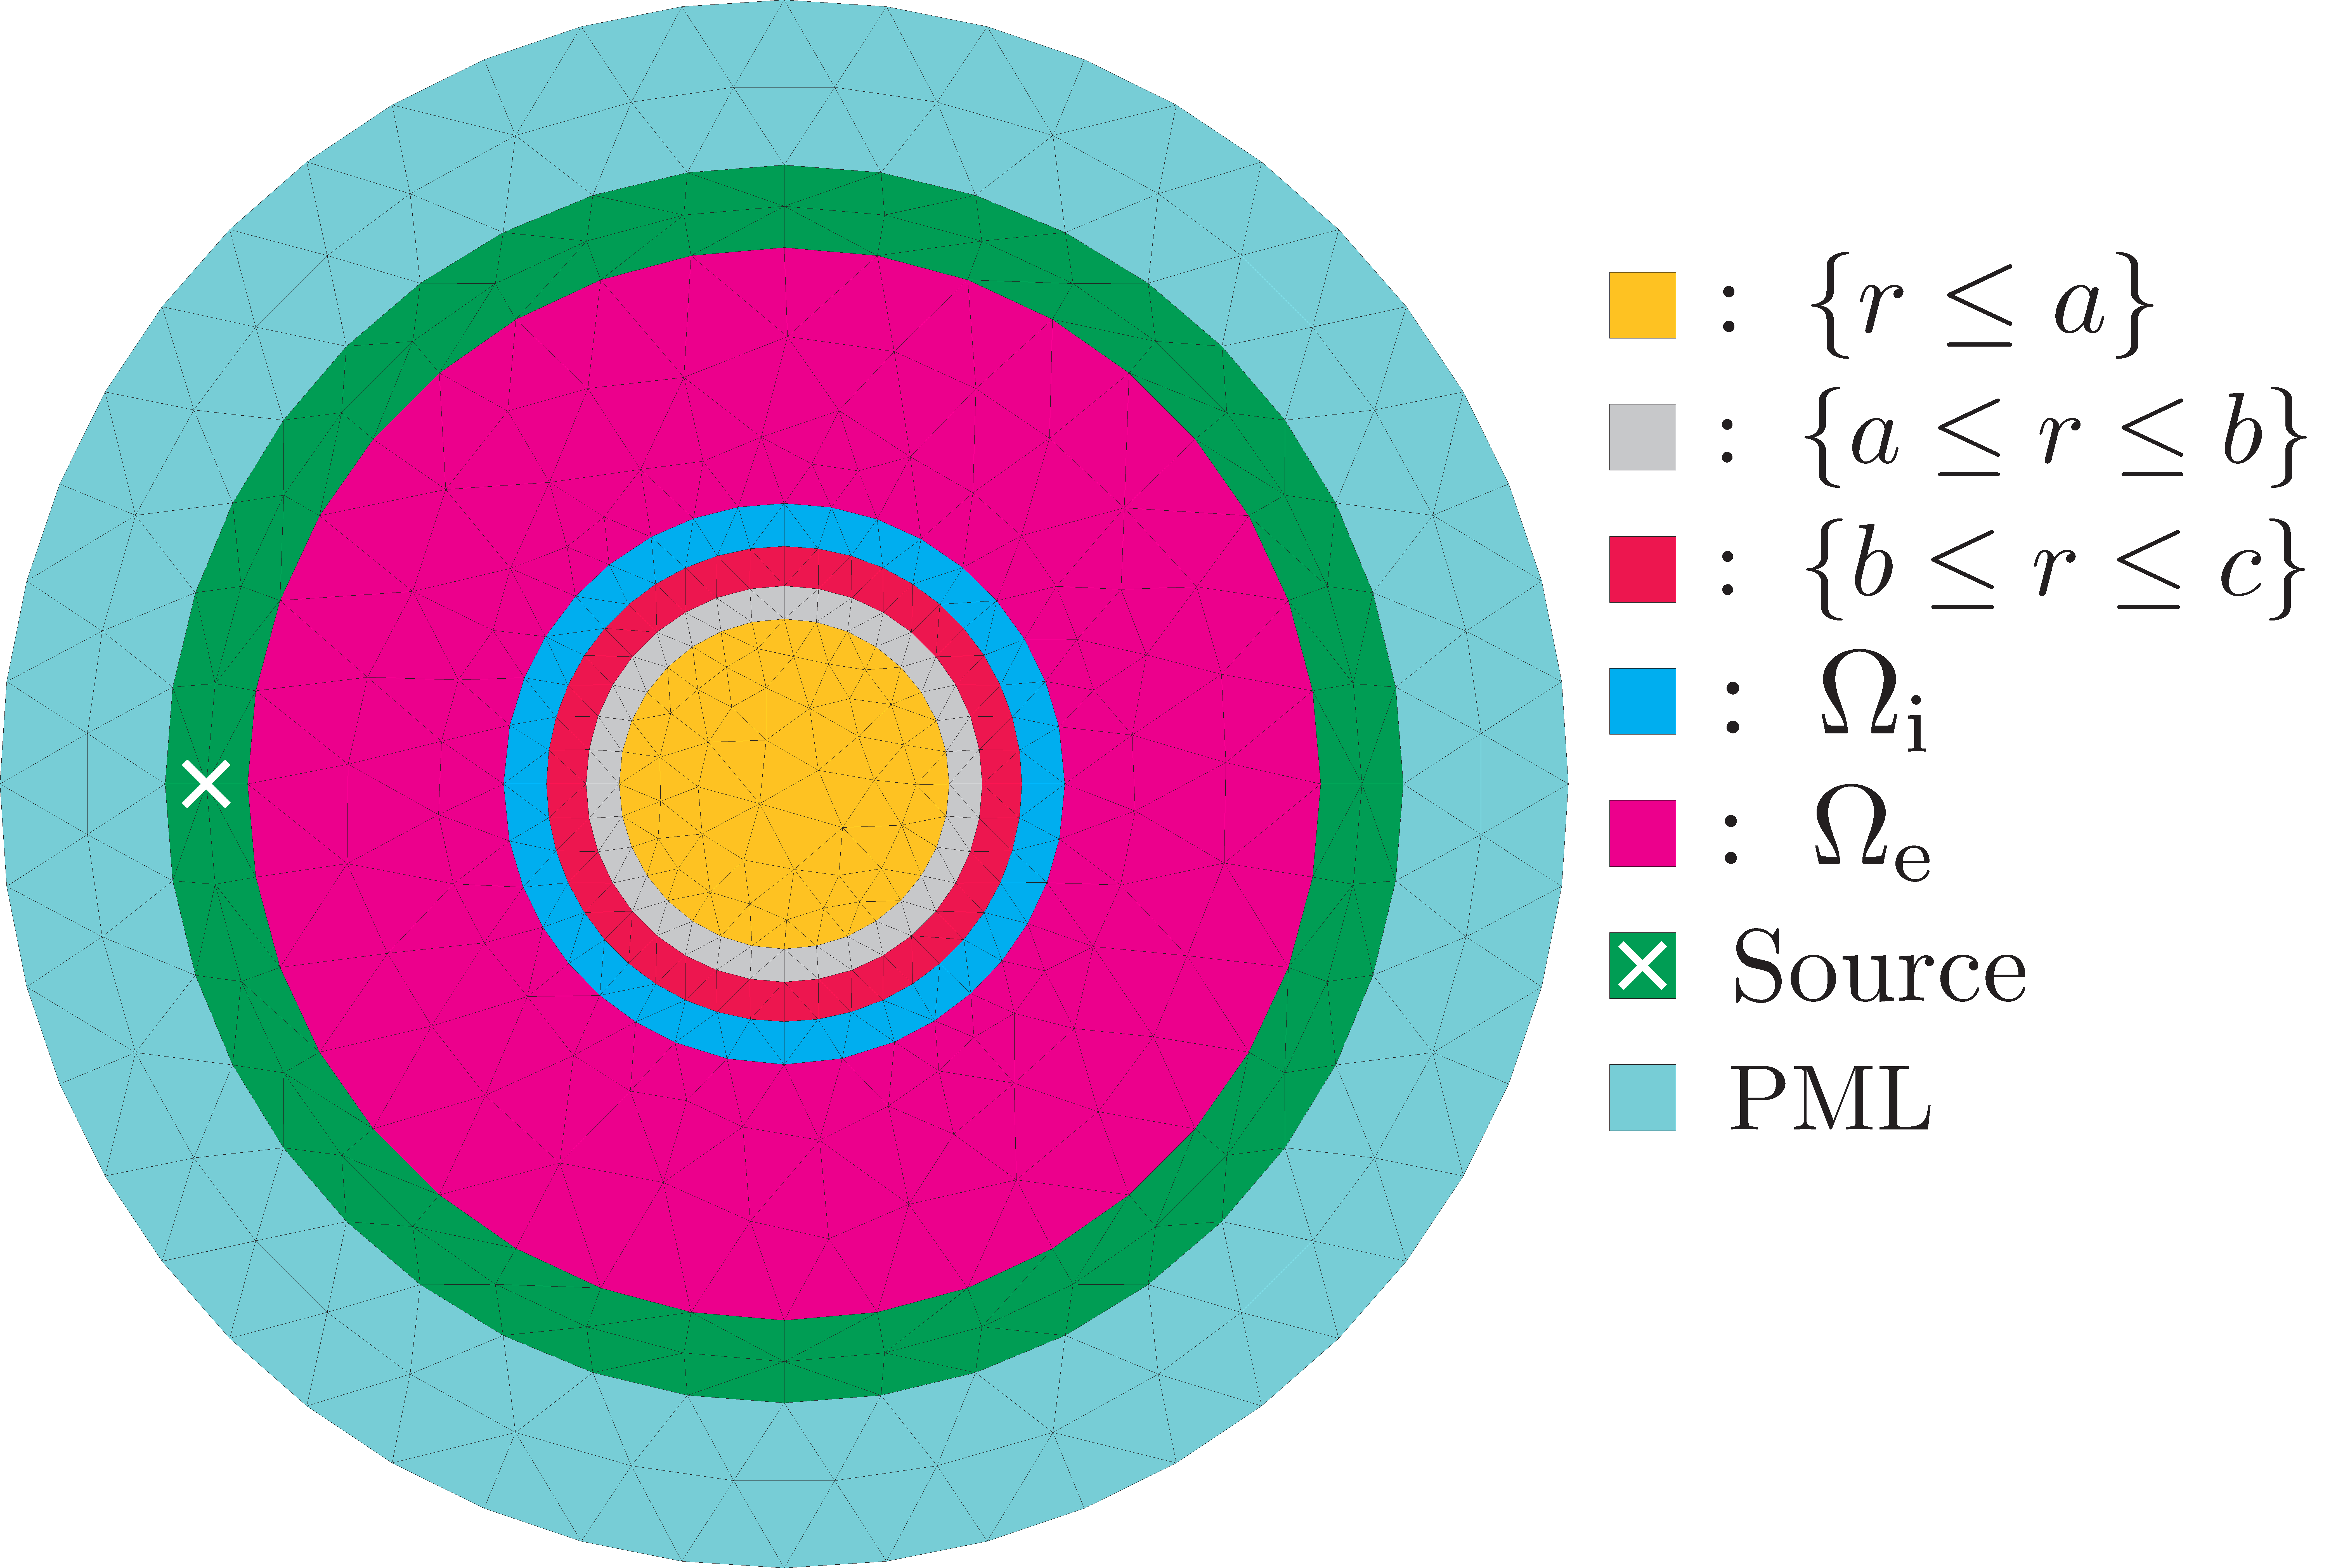
\includegraphics[scale = 0.05]{mesh-MetaMaterial.pdf}}; 
    \node (mypic) at (axis cs:0.69,3.2e-1) {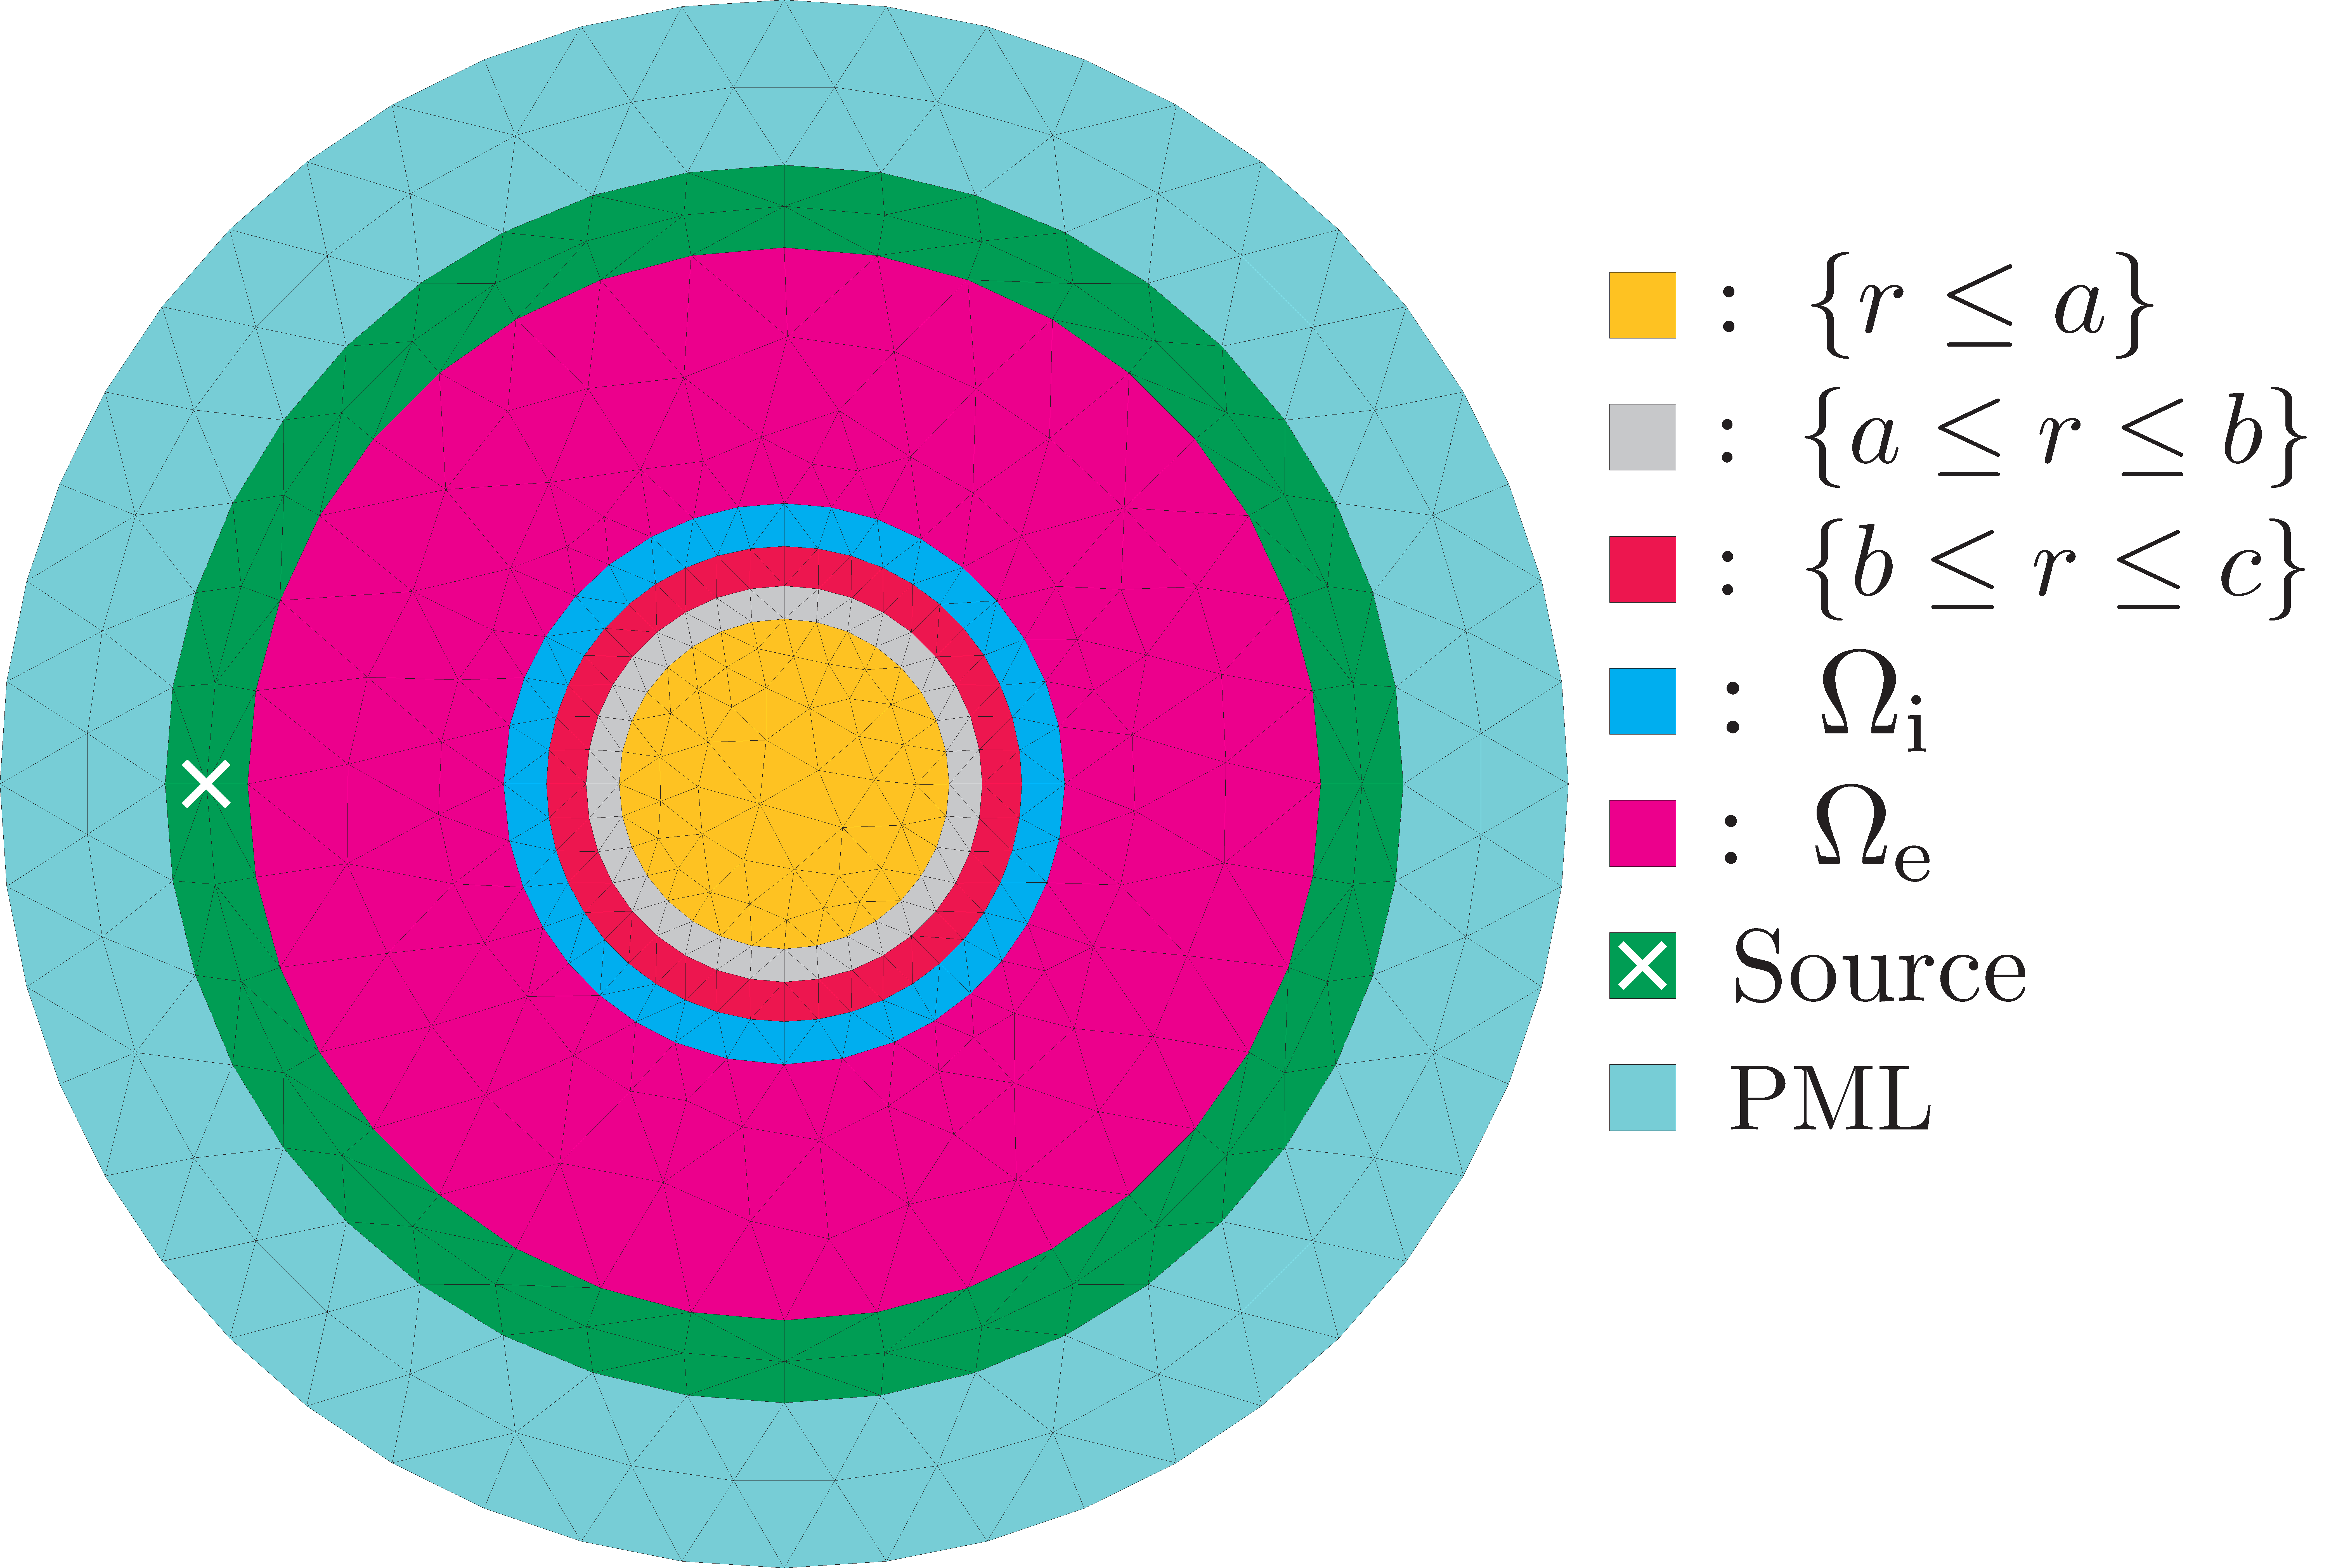
\includegraphics[scale = 0.048]{mesh-MetaMaterial.pdf}}; 
    %mesh-MetaMaterial.pdf

    \nextgroupplot[ 
    xmode=log,
    ymode=log,
    %xmin=0,xmax=1.6e4,
    %xtick={25, 125, 250, 500, 800, 1000},
    %axis x line*=middle,
    %axis y line=middle, 
    ymin = 8e-4,
    ymax = 7e0,
    %width=9cm,
    %restrict y to domain=-4e2:4e2,
    %xtick={0,2e3,4e3,6e3,8e3,10e3,12e3,14e3},
    xlabel= { $h$ },
    legend pos = south east,
    x label style={at={(axis description cs:0.45,+0.175)},anchor=east},
	title = {  $k=2$},
	]

    \addplot[ cyan,ultra thick,dashed,mark=x,mark options={scale=0.35}]  
	table[x=h,y= Galerkin-inner] {../data/MetaMaterial-k2.dat};   
    \addplot[ cyan,ultra thick,mark=x,mark options={scale=0.35}]  
	table[x=h,y=Hybridstab-inner] {../data/MetaMaterial-k2.dat};  
    \addplot[ magenta,only marks,mark=x,mark options={scale=1.2} ]  
	table[x=h,y= Galerkin-outer] {../data/MetaMaterial-k2.dat};   
    \addplot[ magenta,only marks,mark=o,mark options={scale=1} ]  
	table[x=h,y=Hybridstab-outer] {../data/MetaMaterial-k2.dat};  
    \addplot[lightgray,dashed,ultra thick] 
	table[mark=none,x=h,y expr ={3*\thisrowno{0}*\thisrowno{0}}] {../data/MetaMaterial-k2.dat};  
    \legend{ Galerkin $\Omega_{\mathrm{i}}$, Stabilized $\Omega_{\mathrm{i}}$ , Galerkin $\Omega_{\mathrm{e}}$, Stabilized $\Omega_{\mathrm{e}}$, $\mathcal{O}(h^2) $ } 
    
    \nextgroupplot[ 
    xmode=log,
    ymode=log,
    %xmin=0,xmax=1.6e4,
    %xtick={25, 125, 250, 500, 800, 1000},
    %axis x line*=middle,
    %axis y line=middle, 
    ymin = 3e-4,
    ymax = 3e0,
    %width=9cm,
    %restrict y to domain=-4e2:4e2,
    %xtick={0,2e3,4e3,6e3,8e3,10e3,12e3,14e3},
    xlabel= { $h$ },
    legend pos = south east,
    %legend style = { column sep = 10pt, legend columns = 1, legend to name = grouplegend,},
    x label style={at={(axis description cs:0.45,+0.175)},anchor=east},
	title = {  $k=3 $ },
    %legend style={at={(0.5,-0.1)},anchor=north},
	]

    \addplot[ cyan,ultra thick,dashed,mark=x,mark options={scale=0.35}  ,forget plot]  
	table[x=h,y= Galerkin-inner] {../data/MetaMaterial-k3.dat};   
    \addplot[cyan,ultra thick,mark=x,mark options={scale=0.35}  ,forget plot]  
	table[x=h,y=Hybridstab-inner] {../data/MetaMaterial-k3.dat};  
    \addplot[magenta,only marks,mark=x,mark options={scale=1.2}   ,forget plot]  
	table[x=h,y= Galerkin-outer] {../data/MetaMaterial-k3.dat};   
    \addplot[magenta,only marks,mark=o,mark options={scale=1}   ,forget plot]  
	table[x=h,y=Hybridstab-outer] {../data/MetaMaterial-k3.dat};  
    \addplot[lightgray,dashed,ultra thick] 
	table[mark=none,x=h,y expr ={1.3*\thisrowno{0}*\thisrowno{0}*\thisrowno{0}  }] {../data/MetaMaterial-k3.dat};  
    \legend{ $\mathcal{O}(h^3) $ } 

    \nextgroupplot[ 
    xmode=log,
    ymode=log,
    %xmin=0,xmax=1.6e4,
    %xtick={25, 125, 250, 500, 800, 1000},
    %axis x line*=middle,
    %axis y line=middle, 
    ymin = 5e-5,
    ymax = 3e0,
    %width=9cm,
    %restrict y to domain=-4e2:4e2,
    %xtick={0,2e3,4e3,6e3,8e3,10e3,12e3,14e3},
    xlabel= { $h$ },
    legend pos = south east,
    %legend style = { column sep = 10pt, legend columns = 1, legend to name = grouplegend,},
    x label style={at={(axis description cs:0.45,+0.175)},anchor=east},
	title = {  $k=4 $ },
    %legend style={at={(0.5,-0.1)},anchor=north},
	]

    \addplot[ cyan,ultra thick,dashed,mark=x,mark options={scale=0.35}  ,forget plot]  
	table[x=h,y= Galerkin-inner] {../data/MetaMaterial-k4.dat};   
    \addplot[cyan,ultra thick,mark=x,mark options={scale=0.35}  ,forget plot]  
	table[x=h,y=Hybridstab-inner] {../data/MetaMaterial-k4.dat};  
    \addplot[magenta,only marks,mark=x,mark options={scale=1.2}   ,forget plot]  
	table[x=h,y= Galerkin-outer] {../data/MetaMaterial-k4.dat};   
    \addplot[magenta,only marks,mark=o,mark options={scale=1}   ,forget plot]  
	table[x=h,y=Hybridstab-outer] {../data/MetaMaterial-k4.dat};  
    \addplot[lightgray,dashed,ultra thick] 
	table[mark=none,x=h,y expr ={0.4*\thisrowno{0}*\thisrowno{0}*\thisrowno{0}*\thisrowno{0} }] {../data/MetaMaterial-k4.dat};  
    \legend{ $\mathcal{O}(h^4) $ } 

    \end{groupplot}

    %\node at ($(group c1r1) + (-0.0cm,-4.15cm)$) {\ref{grouplegend}}; 
\end{tikzpicture}
\end{document}





